\section*{The Powder Toy Tutorial}
\label{powdertoytutorial}
\NewsAuthor{Sebastian Krähsmaier}

\textbf{Sebastian Krähsmaier (12 J) lernt gerade besucht die Programmiersprache Python bei \href{http://spielend-programmieren.at}{\textit{spielend-programmieren [1]}} und erforscht mittels \textit{The Powder Toy [2]} physikalische Zusammenhänge. In diesem Tutorial versucht er die Aufgabe zu lösen, Wasser von einem Topf links in einen Topf rechts zu befördern.}

\begin{center}
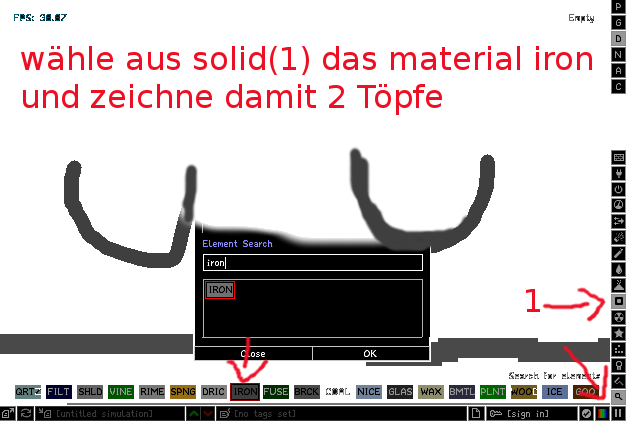
\includegraphics[width=\linewidth]{powdertoytutorial/powdertoytutorial1.png}
\end{center}

\begin{center}
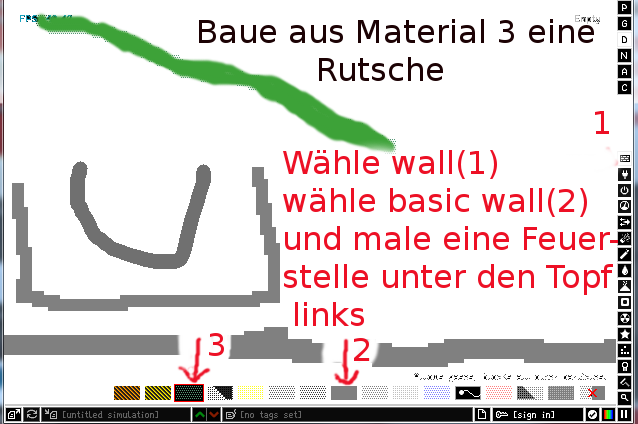
\includegraphics[width=\linewidth]{powdertoytutorial/powdertoytutorial2.png}
\end{center}

\begin{center}
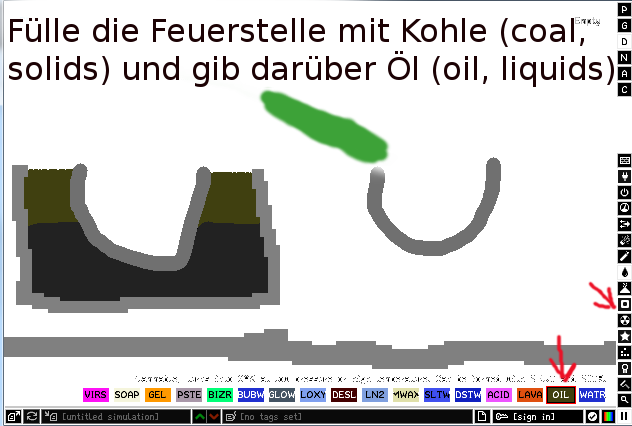
\includegraphics[width=\linewidth]{powdertoytutorial/powdertoytutorial3.png}
\end{center}

\begin{center}
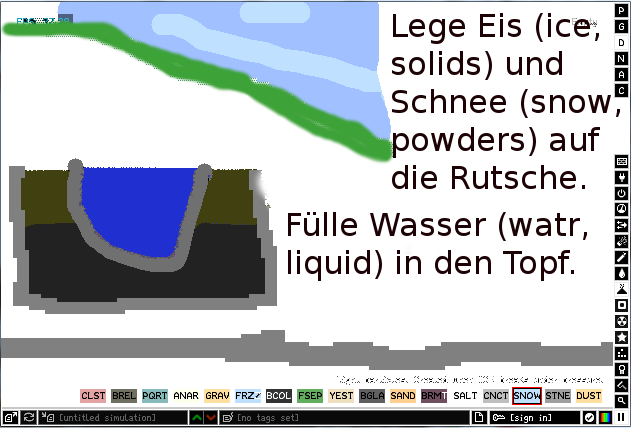
\includegraphics[width=\linewidth]{powdertoytutorial/powdertoytutorial4.png}
\end{center}

\begin{center}
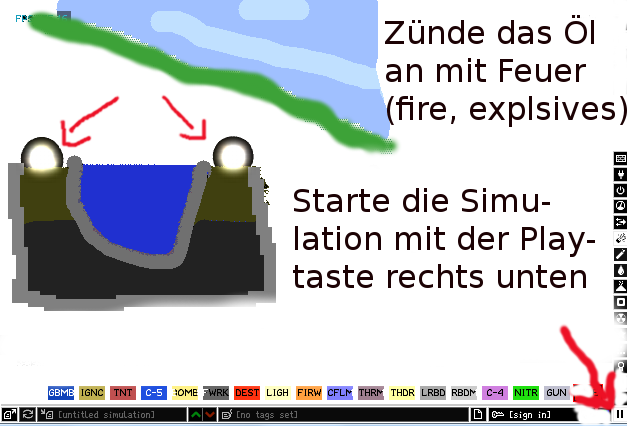
\includegraphics[width=\linewidth]{powdertoytutorial/powdertoytutorial5.png}
\end{center}

Erklärung: Die Flammen sollten das Öl anzünden und anschließend die Kohlen unter dem Metalltopf links. Da Metall wärmeleitend ist steigt aus dem Topf Wasserdampf auf. Die Rutsche über dem Topf ist dampfdurchlässig, der Dampf schmilzt den Schnee und das Eis. Da die Rutsche Flüssigkeiten abweist und nach rechts geneigt ist rinnt das Schmelzwasser in den Topf rechts. Hat man alles richtig gemacht dann verdampft das Wasser im linken Topf komplett und es sammelt sich Wasser im rechten Topf.

\subsection*{Lizenz, Quellen:}
\begin{wrapfigure}{l}{2.0cm}

\includegraphics[width=2cm]{powdertoytutorial/ccbysa88x31.png}
\end{wrapfigure}
Dieses Material steht unter der Creative-Commons-Lizenz Namensnennung - Weitergabe unter gleichen Bedingungen 4.0 International. Um eine Kopie dieser Lizenz zu sehen, besuchen Sie \url{http://creativecommons.org/licenses/by-sa/4.0/deed.de}.

\subsection*{Download, Feedback:}
\footnotesize{
Ordner \texttt{powdertoytutorial} \Mundus\ \href{http://spielend-programmieren.at/risjournal/001}{spielend-programmieren.at/risjournal/001}\\
Startseite: \href{http://spielend-programmieren.at/de:ris}{spielend-programmieren.at/de:ris}\\ 
\Letter\:  horst.jens@spielend-programmieren.at \\}
\normalsize{}

\textbf{Quellen:} \\
{[}1{]} \href{http://spielend-programmieren.at}{spielend-programmieren.at} \\
{[}2{]} \href{http://powdertoy.co.uk/}{powdertoy.co.uk/} \\
